\section{Background}

% \begin{frame}{The Circuit Model of Quantum Computation}

% Dirac notation: $\ket{0} = \begin{bmatrix} 1 \\ 0 \end{bmatrix}$, $\ket{1} = \begin{bmatrix} 0 \\ 1 \end{bmatrix}$.

% \vspace{0.5cm}

% \begin{center}

% \begin{tikzpicture}[remember picture]
% \node (C) [inner sep=0pt, outer sep=0pt] {
% \begin{quantikz}[row sep=0.55cm, column sep=0.45cm]
% \lstick{$\ket{\psi_1}$} & \gate{U_1} & \meter{} \\
% \lstick{$\ket{\psi_2}$} & \gate{U_2} & \meter{}
% \end{quantikz}
% };
% \end{tikzpicture}

% \begin{tikzpicture}[remember picture,overlay]
% \coordinate (NW) at ($(C.north west)$);
% \coordinate (NE) at ($(C.north east)$);
% \coordinate (SW) at ($(C.south west)$);
% \coordinate (SE) at ($(C.south east)$);

% \only<2->{%
% \draw[decorate,decoration={brace,amplitude=5pt},thick]
%   ($(SW)+(-0.2,0)$) -- ($(NW)+(-0.2,0)$)
%   node[midway,xshift=-1cm,align=left,text width=5.6cm]
%   {\textbf<2->{qubit\\}
%    $\ket{\psi}\in\mathbb{C}^2, $\\
%    $\ket{\psi}=\alpha\ket{0}+\beta\ket{1}, $\\
%    $|\alpha|^2+|\beta|^2=1$.};
% }

% \only<3->{%
% \draw[decorate,decoration={brace,amplitude=5pt,mirror},thick]
%   ($(SW)+(+1,-0.2)$) -- ($(SE)+(-1.1,-0.2)$)
%   node[midway,yshift=-0.95cm,align=left,text width=4cm]
%   {\textbf<3->{gate}\\
%    $U\in\mathbb{C}^{2\times 2}$\\
%   $U^\dagger U=I$ (unitary)};
% }

% \only<4->{%
% \draw[decorate,decoration={brace,amplitude=5pt,mirror},thick]
%   ($(SE)+(0.2,0)$) -- ($(NE)+(0.2,0)$)
%   node[midway,xshift=4cm,align=left,text width=6.2cm]
%   {\textbf<4->{measurement}\\
%    $b \in \{\ket{0},\ket{1}\}$\\
%    $\Pr(b) = |\langle b\mid\psi\rangle|^2$.\\
%    Works for any \\orthonormal basis\\of $\mathbb{C}^2$.};
% }
% \end{tikzpicture}

% \end{center}

% \vspace{1.5cm}

% \only<5->{%
% Composition between gates is by $\otimes$ to preserve linearity.
% }

% \end{frame}

\begin{frame}{Measurement-Based Quantum Computation (MBQC)}

\begin{tikzpicture}[remember picture]

\node (C) [inner sep=0pt, outer sep=0pt, anchor=west] at (0,0) {
\begin{quantikz}[row sep=0.45cm, column sep=0.45cm, wire types={q,n,q}]
\lstick{$\ket{0}$} & \gate[3]{C} & \meter{} \\
\lstick{$\vdots$}       &             & \vdots   \\
\lstick{$\ket{0}$} &             & \meter{}
\end{quantikz}
};

\only<2->{%
\draw[->, thick]
  ($(C.east)+(0.6,0)$) -- ($(C.east)+(3.2,0)$)
  coordinate[midway] (Amid);
}

\only<2->{%
\node[anchor=south] at ($(Amid)+(0,0.12)$)
{\scriptsize\textbf{MBQC}};
}

\node (B) [anchor=west] at ($(C.east)+(3.5,0)$) {
\only<3->{%
\begin{minipage}{0.4\linewidth}
\begin{itemize}\small
\item Single-qubit measurements on a
\item "resource state"
\item <4-> Excluding resource state, done in constant depth.
\end{itemize}
\end{minipage}
}
};
\end{tikzpicture}

\end{frame}

\begin{frame}{Example Resource State: Graph State}

Let $G = (V,E)$ be a graph. The \textbf{graph state} $\ket{G}$ has 
\begin{itemize}
    \item For every $v \in V$, prepare a qubit $\ket+ = H \ket0$.
    \item For every $e = (u,v) \in E$, apply $CZ$ on qubits of $u$ and $v$.
\end{itemize}

\vspace{0.5cm}

\only<2->{%
\makebox[\textwidth][c]{%
\begin{minipage}{0.3\textwidth}
\centering
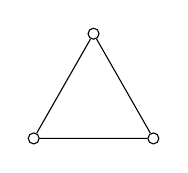
\begin{tikzpicture}[scale=0.95, every node/.style={circle,draw,inner sep=1.4pt}]
\node (a) at (0,0.9) {};
\node (b) at (-0.8,-0.5) {};
\node (c) at (0.8,-0.5) {};
\draw (a)--(b)--(c)--(a);
\end{tikzpicture}
\end{minipage}
\hspace{0.4cm}
\begin{minipage}{0.3\textwidth}
\centering
\begin{tikzpicture}
\node [inner sep=0pt, outer sep=0pt] {
\begin{quantikz}[row sep=0.42cm, column sep=0.28cm, cells={inner sep=1pt}]
\lstick{$\ket{0}$} & \gate{H} & \ctrl{1}  & \ctrl{2}  & \qw      \\
\lstick{$\ket{0}$} & \gate{H} & \ctrl{-1} & \qw       & \ctrl{1} \\
\lstick{$\ket{0}$} & \gate{H} & \qw       & \ctrl{-2} & \ctrl{-1}
\end{quantikz}
};
\end{tikzpicture}
\end{minipage}
}%
}

\end{frame}

\begin{frame}{Grid Graph State}

Let $\Grid_{m \times n}$ be the grid graph with $m$ rows and $n$ columns. \\
Let $\ket{\Grid_{m \times n}}$ be its graph state. 

\vspace{0.5cm}

\only<2->{Example: $\ket{\Grid_{2 \times 3}}$.}

\vspace{0.5cm}

\only<2->{%
\makebox[\textwidth][c]{%
\begin{minipage}{0.3\textwidth}
\centering
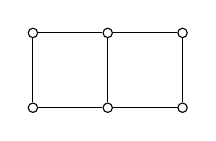
\begin{tikzpicture}[scale=0.95, every node/.style={circle,draw,inner sep=1.2pt}]
\node (a1) at (0,1) {};
\node (a2) at (1,1) {};
\node (a3) at (2,1) {};
\node (b1) at (0,0) {};
\node (b2) at (1,0) {};
\node (b3) at (2,0) {};
\foreach \u/\v in {a1/a2,a2/a3,b1/b2,b2/b3,a1/b1,a2/b2,a3/b3} \draw (\u)--(\v);
\end{tikzpicture}
\end{minipage}%
\hspace{0.35cm}%
\begin{minipage}{0.3\textwidth}
\centering
\begin{tikzpicture}
\node (Cgrid) [inner sep=0pt, outer sep=0pt] {
\begin{quantikz}[row sep=0.34cm, column sep=0.22cm, cells={inner sep=0.8pt}]
\lstick{$\ket{+}$} & \ctrl{1}  & \ctrl{2}  & \qw       & \qw       \\
\lstick{$\ket{+}$} & \ctrl{-1} & \qw       & \ctrl{2}  & \qw       \\
\lstick{$\ket{+}$} & \ctrl{1}  & \ctrl{-2} & \qw       & \ctrl{2}  \\
\lstick{$\ket{+}$} & \ctrl{-1} & \ctrl{2}  & \ctrl{-2} & \qw       \\
\lstick{$\ket{+}$} & \ctrl{1}  & \qw       & \qw       & \ctrl{-2} \\
\lstick{$\ket{+}$} & \ctrl{-1} & \ctrl{-2} & \qw       & \qw       
\end{quantikz}
};
\end{tikzpicture}
\end{minipage}%
}%
}

\end{frame}

\begin{frame}{Universal Resource, Informally}

\begin{definition}
Let $\LO$ denote local operations, i.e. single qubit unitaries and measurements. Let $\CC$ denote classical communication.
\end{definition}

\begin{definition}<2->
Let $\Psi$ be a family of resource states. $\Psi$ is a \textbf{universal resource} for MBQC if for every $U \in SU(2^n)$, $\forall n \in \mathbb{N}$, there is a sequence of $\LOCC$ and some resource state $\ket\psi \in \Psi$, such that 
\begin{align}
    \ket{\psi} \xrightarrow{\LOCC} U \ket{0^n}
\end{align}
\only<3->{%
In other words, we can ``simulate any state'' using $\LOCC$ and a resource state from $\Psi$.
}
\end{definition}

\end{frame}

\begin{frame}{Grid is a Universal Resource}

\begin{theorem}
$\{\Grid_{1 \times i}\}_{i\in \mathbb{N}}$ (The lines) are a 1-qubit universal resource for MBQC.
\end{theorem}

\begin{lemma}[Euler decomposition]
Every single-qubit unitary can be expressed (up to global phase) as the product
\begin{align}
    R_z(\theta_3)R_x(\theta_2)R_z(\theta_1)
\end{align}
for some $\theta_1, \theta_2, \theta_3 \in [0,2\pi]$.
\end{lemma}

\begin{lemma}
$R_x(\theta) = H R_z(\theta) H$, for all $\theta \in [0,2\pi]$.
\end{lemma}

\end{frame}

\begin{frame}{Grid is a Universal Resource cont'd}

\begin{proof}[Informal proof.]
\vspace{-0.8cm}
\begin{align}
\begin{quantikz}[row sep=0.2cm, column sep=0.2cm]
\lstick{$\ket{\phi}$} & \ctrl{1}  & \gate{R_z(\theta)} & \gate{H} & \meter{} \\
\lstick{$\ket{+}$}    & \ctrl{-1} & \qw      &          &
\end{quantikz}
\;=\;
\begin{quantikz}[row sep=0.2cm, column sep=0.2cm]
\lstick{$\ket{+}$}              & \ctrl{1}  & \meter{} \\
\lstick{$HR_z{\theta}\ket\phi$} & \targ{}   & \qw
\end{quantikz}
\end{align}
\only<2->{%
If we measure $0$, we get $HR_z(\theta)\ket\phi$ in the second register. If we measure $1$, we get $XH_z(\theta)\ket\phi$. Thus given the right measurements we can apply any 1-qubit gate by repeating the construction:
}
\only<3->{%
\begin{center}
\begin{quantikz}[row sep=0.1cm, column sep=0.1cm]
\lstick{$\ket{\phi}$} & \ctrl{1}  & \gate{R_z(\theta_1)} & \gate{H} & \meter{} \\
\lstick{$\ket{+}$}    & \ctrl{-1} & \ctrl{1}      & \gate{R_z(\theta_2)} & \gate{H} & \meter{} \\
\lstick{$\ket{+}$}    & \qw       & \ctrl{-1}     & \qw & \qw & \qw & \qw \\
\end{quantikz}
\end{center}
}
\end{proof}

\end{frame}

\begin{frame}{Grid is a Universal Resource cont'd}

\begin{theorem}
Let $\Grid$ denote the family of all grid graphs. $\Grid$ is a universal resource for MBQC.
\end{theorem}

\begin{proof}
Similar to the proof for the line.
\end{proof}

\end{frame}

\begin{frame}{Comparability Grid}

\begin{definition}
Let $\CGrid_{m \times n}$ denote the $m$ rows, $n$ column \textbf{comparability grid}, which is an undirected graph $G = (V,E)$ with
\begin{align}
    V &= \{(i,j) \mid i \in [m], j \in [n]\} \\
    E &= \{ \{(i_1,j_1),(i_2,j_2)\} \mid (i_1,j_1),(i_2,j_2) \in V, i_2 \geq i_1, j_2 \geq j_1. \}
\end{align}  
i.e. the grid with partial order $\leq$ defining edges.
\end{definition}

\end{frame}

\begin{frame}{Comparability Grid Example}

Example: $\CGrid_{3 \times 3}$:

\vspace{0.5cm}

\centering
\begin{tikzpicture}[
  scale=1.7,
  every node/.style={circle, fill=black, inner sep=1.5pt},
  edge/.style={line width=0.5pt}
]
\node (v11) at (1,1) {};
\node (v12) at (1,2) {};
\node (v13) at (1,3) {};
\node (v21) at (2,1) {};
\node (v22) at (2,2) {};
\node (v23) at (2,3) {};
\node (v31) at (3,1) {};
\node (v32) at (3,2) {};
\node (v33) at (3,3) {};

\draw[edge] (v11) -- (v12);
\draw[edge] (v11) -- (v21);
\draw[edge] (v11) -- (v22);
\draw[edge] (v11) -- (v23);
\draw[edge] (v11) -- (v32);

\draw[edge] (v12) -- (v13);
\draw[edge] (v12) -- (v22);
\draw[edge] (v12) -- (v23);

\draw[edge] (v13) -- (v23);

\draw[edge] (v21) -- (v22);
\draw[edge] (v21) -- (v31);
\draw[edge] (v21) -- (v32);

\draw[edge] (v22) -- (v23);
\draw[edge] (v22) -- (v32);

\draw[edge] (v23) -- (v33);
\draw[edge] (v31) -- (v32);
\draw[edge] (v32) -- (v33);

\draw[edge] (v11) to[bend left=20] (v13);
\draw[edge] (v21) to[bend left=20] (v23);
\draw[edge] (v31) to[bend left=20] (v33);

\draw[edge] (v11) to[bend right=20] (v31);
\draw[edge] (v12) to[bend right=20] (v32);

\draw[edge] (v11) to[bend right=20] (v33);
\draw[edge] (v12) -- (v33);
\draw[edge] (v13) to[bend right=20] (v33);

\draw[edge] (v21) -- (v33);
\draw[edge] (v22) to (v33);

\node[draw=none, fill=none, inner sep=0pt, anchor=east] at ($(v13)+(-0.15,0)$) {$ (1,3)$};
\node[draw=none, fill=none, inner sep=0pt, anchor=west] at ($(v33)+(0.15,0)$) {$ (3,3)$};
\node[draw=none, fill=none, inner sep=0pt, anchor=east] at ($(v11)+(-0.15,0)$) {$ (1,1)$};
\node[draw=none, fill=none, inner sep=0pt, anchor=west] at ($(v31)+(0.15,0)$) {$ (3,1)$};
\end{tikzpicture}

\end{frame}